\section{Korlátok}
	Érdekes kérdés, hogy egy ilyen böngészőből használt, webes alapú adatmegjelenítő eszköz mennyire bír el nagyobb mennyiségű adat megjelenítésével. A következőkben az x-y pont grafikon terhelhetőségét vizsgálom. 
	
	\subsection{Törékenység}
	Több azonos teszt futtatása közben szerettem volna használni, az adatok újratöltése funkciót, hogy minden alkalommal ugyan azt a grafikont jelenítse meg, csak egyre nagyobb adathalmazzal. De sajnálatos módon ezt a funkciót nem sikerült működésre bírni egy idő után, azonban a produkált egy hosszú hibaüzenetet, ami a \ref{fig:hibaorenz}. ábrán látszik.
	\begin{figure}[h!]
		\centering
		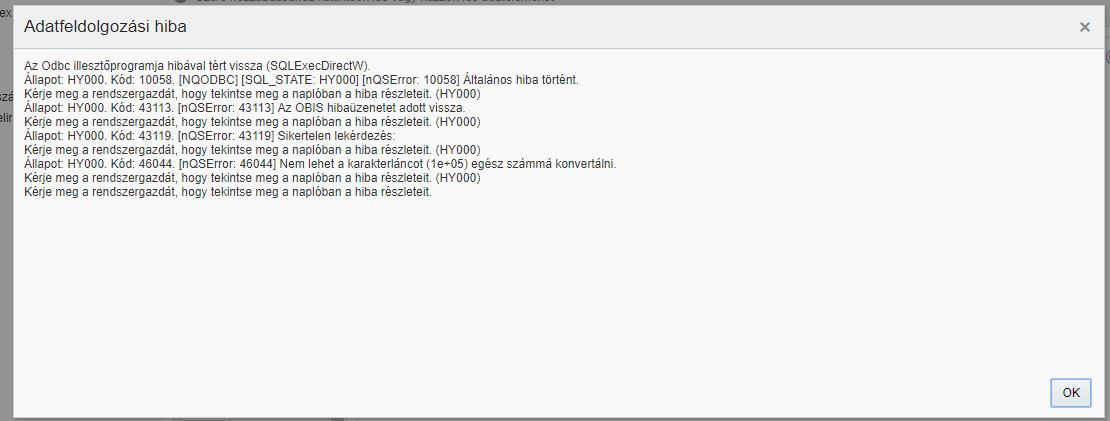
\includegraphics[width=1.0\linewidth]{dani_imgs/hiba_orenz}
		\caption{Adatok újratöltése után konverziós problémával elbukott megjelenítés}
		\label{fig:hibaorenz}
	\end{figure}

	\subsection{Megjelenítési korlát}
	A megjeleníthető adatok számának van egy (nem specifikált) felső korlátja. Például az X-Y ponthalmaz megjelenítője nem képes már 3x100k adat megjelenítésére, ekkor a \ref{fig:hiba}. ábrán látható hibaüzenetet produkálja. Emiatt, lényegében hamarabb akad meg a megjelenítés mintsem kifagyna az oldal a kezdeti megjelenítés előtt.
	\begin{figure}[h!]
		\centering
		
\includegraphics[width=1.0\linewidth]{dani_imgs/hiba}
		\caption{Túl sok betöltött adat által generált hiba}
		\label{fig:hiba}
	\end{figure}
	
	
	\subsection{Teszt adatok : Lorentz attraktor}
	Tesztadatként a lorentz attraktor x-y értékeit használtam. Mivel ez egy szinte végtelenségig futtatható számítás, tetszőleges mennyiségű x-y-z koordináta rendszerben vizualizálható látványos adathalmaz az eredmény. Nagyjából 38640 x, y és index-ből felépülő megjelenítés a \ref{fig:lorenztxy}. ábrán látható. Ennyi adat esetén a megjelenítés még viszonylag gyorsan megtörténik, azonban bármilyen funkció ami manipulációval jár (pl. zoomolás) eszméletlenül lassú, és sajnos megakasztja a böngészőt is (lásd: \ref{fig:kifagyott}). Ezáltal elmondható, hogy ez az eszköz nem kifejezetten alkalmas sok egyedi adat egyszerre történő megjelenítésére és vizualizációjára. 
	\begin{figure}
		\centering
		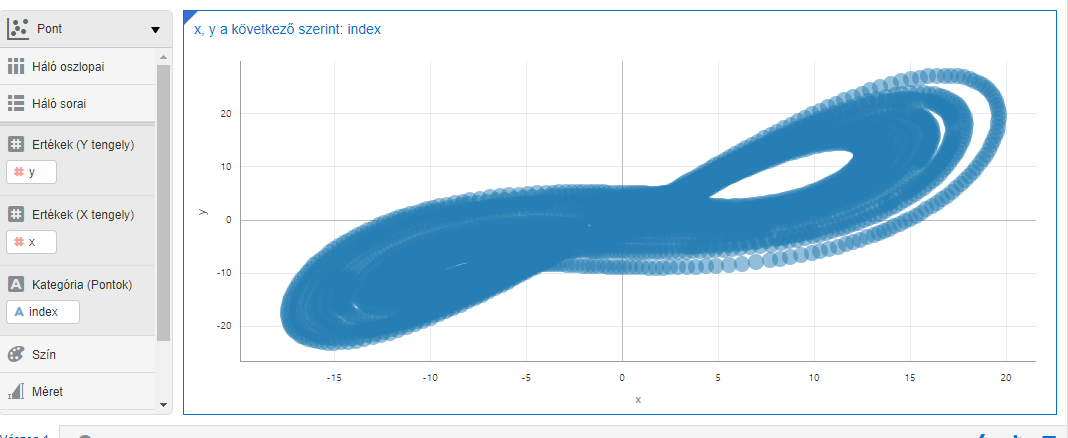
\includegraphics[width=1.0\linewidth]{dani_imgs/lorenzt_xy}
		\caption{Lorentz attraktor X-Y}
		\label{fig:lorenztxy}
	\end{figure}

	\begin{figure}
		\centering
		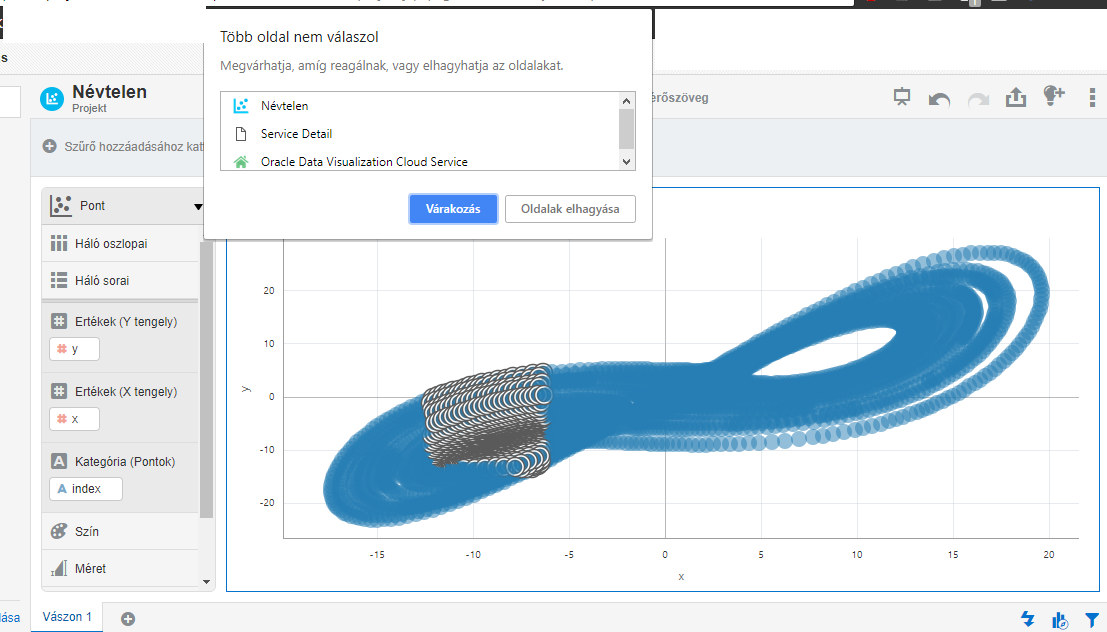
\includegraphics[width=1.0\linewidth]{dani_imgs/kifagyott}
		\caption{Nagy adathalmaz esetén a Zoomolás miatt összeomlik az oldal}
		\label{fig:kifagyott}
	\end{figure}
	
	